\documentclass[a4paper,12pt]{article}

\usepackage{Packages}
\usepackage{breqn}
\usepackage{amsmath}
\usepackage{resizegather}
\long\def\/*#1*/{}

\begin{document}
%included in part 1
\tableofcontents %included in part 1
\newpage

\section{PCA and Isomap}
\subsection{a}
The first two principle components of PCA for all classes are:
\begin{figure}[H]
\hfill
\makebox[\textwidth][c]{{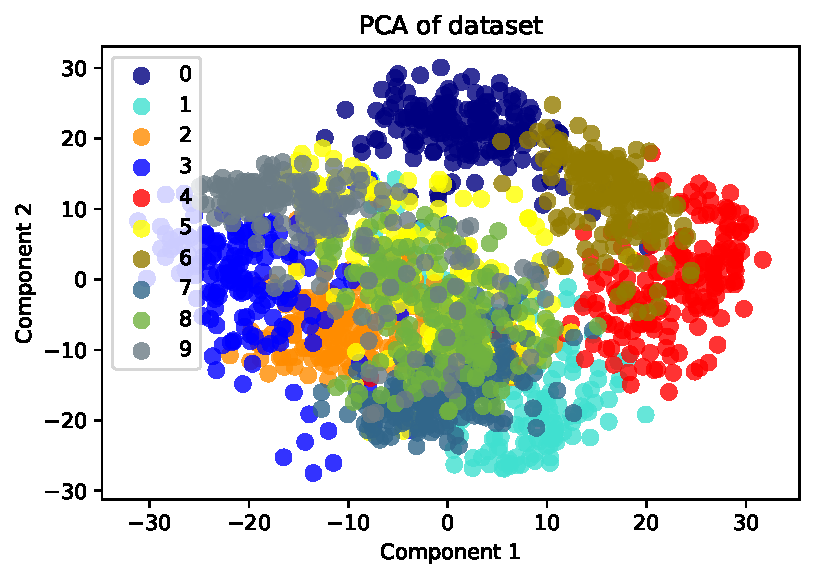
\includegraphics[width=12cm]{./Figures/output_4_1}}}
\hfill
\caption{Scatter plot for the first two principal components}
\label{fig:a}
\label{41}
\end{figure}

The classes are not very well separated. 

\subsection{b}
The manifold is constructed using the isomap with the given conditions. The results are: 
\begin{figure}[H]
\hfill
\makebox[\textwidth][c]{{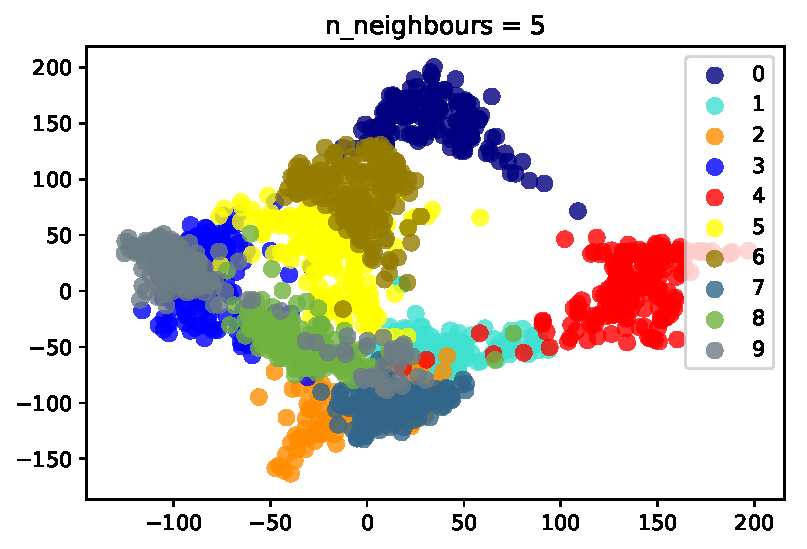
\includegraphics[width=12cm]{./Figures/output_5_1}}}
\hfill
\caption{Scatter plot for aligned data, $n_{neighbours}$ = 5.}
\label{51}
\end{figure}

\begin{figure}[H]
\hfill
\makebox[\textwidth][c]{{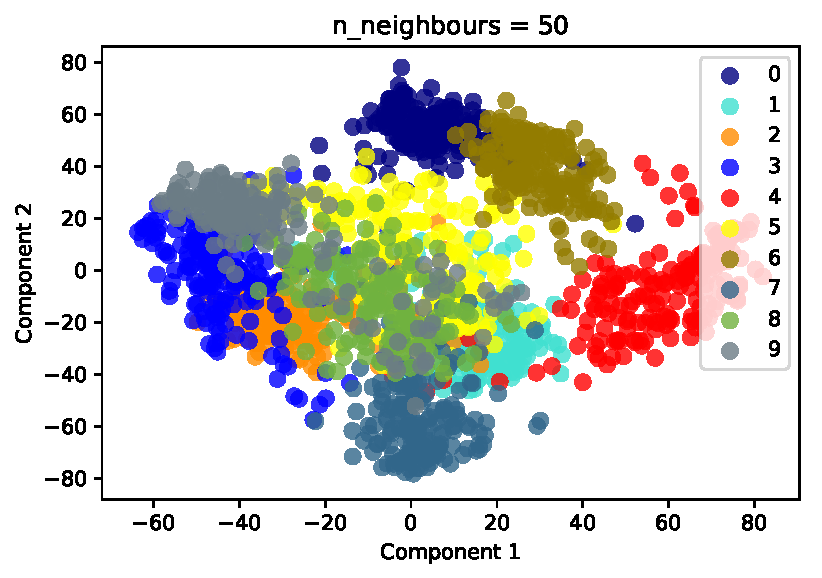
\includegraphics[width=12cm]{./Figures/output_5_2}}}
\hfill
\caption{Scatter plot for aligned data, $n_{neighbours}$ = 50.}
\label{52}
\end{figure}

\begin{figure}[H]
\hfill
\makebox[\textwidth][c]{{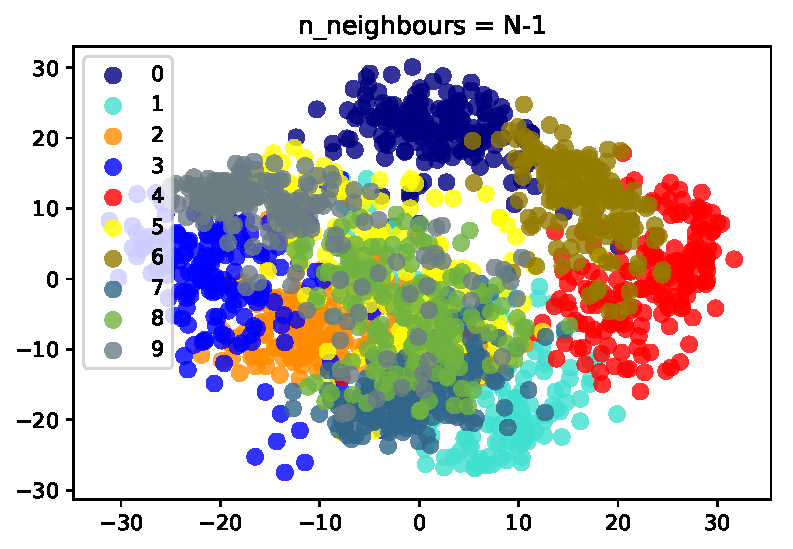
\includegraphics[width=12cm]{./Figures/output_5_3}}}
\hfill
\caption{Scatter plot for aligned data, $n_{neighbours}$ = N-1. }
\label{53}
\end{figure}
\subsection{c}
More neighbours decreases the computed score. As the number of neighbours increases, the separation of the different classes becomes more vague. For $n_{neighbours}=5$ the classes are decently separated, while for $n_{neighbours}=50$ and $n_{neighbours}=N-1$ there is increasingly more overlap. If the 1-norm (score) is zero, it means that the of the transformed dataset is identical to the the reference data (PCA) for one of the 8 transformations.
This is the case when the isomap embedding does not have any effect on the PCA data, as can been seen by comparing figures \ref{fig:a} and \ref{53}. The reason for this is that  all the the neighbours are used the isomap cannot make a manifold. 



\section{Classical multidimensional scaling}
\subsection{a}

\begin{equation}
\begin{aligned}
d_{ij}=||{\bf p_i-p_j}||^2=||{\bf p_i-p_j}||\;||{\bf p_i-p_j}||=2\big \langle{\bf p_i,p_j}\big \rangle+||{\bf p_i}||^2+||{\bf p_j}||^2
\end{aligned}
\end{equation}

\subsection{b}
The explanation is that because the point set is mean-centered the scaling factor vector (${\bf q}$) does not matter.If statement in question b can be proven in 1 direction all the other dimensions are proven too. The proof can be given mathematically by first expanding the sum sign:
\begin{equation}
\begin{aligned}
\sum_{1\leq i \leq n} \big \langle{\bf p_i,q}\big \rangle=p_{1}q+\ldots+p_{n}q=q(p_1+\ldots +p_n)=0
\end{aligned}
\label{eq:statement b}
\end{equation}
The mean-centered definition in respectively all dimensions and one dimension is given by:
\begin{equation}
\begin{aligned}
\sum_{i=1}^n {\bf p_i}={\bf 0 } \rightarrow \sum_{1 \leq i \leq n} (p_1+\ldots +p_n)=0
\end{aligned}
\end{equation}
Therefore equation \ref{eq:statement b} is zero and equation b in the question holds.

\subsection{c}
Prove that:
\begin{equation}
\begin{aligned}
||{\bf p_i}||^2=\sum_{l=1}^n \frac{d_{il}}{n}-\sum^{n}_{k=1}\sum_{l=1}^n\frac{d_{kl}}{2n^2}
\end{aligned}
\label{eq:proven c}
\end{equation}
This equation can be expanded to:
\begin{equation}
\begin{aligned}
||{\bf p_i}||^2=\sum_{l=1}^n \frac{||{\bf p_i-p_l}||^2}{n}-\sum^{n}_{k=1}\sum_{l=1}^n\frac{||{\bf p_k-p_l}||^2}{2n^2}
\end{aligned}
\end{equation}
Which can be written as:
\begin{equation}
\begin{aligned}
||{\bf p_i}||^2=\sum_{l=1}^n \frac{2\big \langle{\bf p_i,p_l}\big \rangle+||{\bf p_i}||^2+||{\bf p_l}||^2}{n}-\sum^{n}_{k=1}\sum_{l=1}^n\frac{2\big \langle{\bf p_k,p_l}\big \rangle+||{\bf p_k}||^2+||{\bf p_l}||^2}{2n^2}
\end{aligned}
\end{equation}
Since equation \ref{eq:statement b} holds this can be rewritten as:
\begin{equation}
\begin{aligned}
||{\bf p_i}||^2=
\sum_{l=1}^n \frac{||{\bf p_i}||^2+||{\bf p_l}||^2}{n}-\sum^{n}_{k=1}\sum_{l=1}^n\frac{||{\bf p_k}||^2+||{\bf p_l}||^2}{2n^2}=
\end{aligned}
\end{equation}
Because ${\bf p_i}$ and ${\bf p_k}$ are added $n$ times, this can be rewritten to:
\begin{equation}
\begin{aligned}
\frac{1}{n}\left(n ||{\bf p_i}||^2 + \sum_{l=1}^n ||{\bf p_l}||^2 \right)-\frac{1}{2n^2} \sum_{k=1}^n \left(n ||{\bf p_k}||^2  + \sum^{n}_{l=1} ||{\bf p_l}||^2 \right)
\end{aligned}
\end{equation}
Vectors ${\bf p_l}$ is added $n$ times, therefore:
\begin{equation}
\begin{aligned}
||{\bf p_i}||^2+\frac{1}{n}\left(\sum_{l=1}^n ||{\bf p_l}||^2 \right)-\frac{1}{2n^2}\left( n \sum_{l=1}^n ||{\bf p_l}||^2+n \sum_{k=1}^n ||{\bf p_k}||^2 \right)
\end{aligned}
\end{equation}
The sum of $k$ and $l$ for these vectors are the same, therefore:
\begin{equation}
\begin{aligned}
||{\bf p_i}||^2+\frac{1}{n}\left(\sum_{l=1}^n ||{\bf p_l}||^2 \right)-\frac{2n}{2n^2}\left(  \sum_{l=1}^n ||{\bf p_l}||^2 \right)=||{\bf p_i}||^2
\end{aligned}
\end{equation}
Now equation \ref{eq:proven c} is shown to be correct. 

\subsection{d}
First the distance is expanded:
\begin{equation}
\begin{aligned}
d_{ij}=||{\bf p_i-p_j}||^2=2\big \langle{\bf p_i,p_j}\big \rangle+||{\bf p_i}||^2+||{\bf p_j}||^2
\end{aligned}
\label{eq:1}
\end{equation}

Now equation \ref{eq:proven c} is substituted in \ref{eq:1} for $||{\bf p_i}||^2$ and $||{\bf p_j}||^2$:
\begin{equation}
\begin{aligned}
d_{ij}=2\big \langle{\bf p_i,p_j}\big \rangle+\sum_{l=1}^n \frac{d_{il}}{n}-\sum^{n}_{k=1}\sum_{l=1}^n\frac{d_{kl}}{n^2}+\sum_{l=1}^n \frac{d_{jl}}{n}
\end{aligned}
\label{eq:2}
\end{equation}
Therefore:
\begin{equation}
\begin{aligned}
-2\big \langle{\bf p_i,p_j}\big \rangle=d_{ij}-\sum_{l=1}^n \frac{d_{il}}{n}-\sum_{l=1}^n \frac{d_{jl}}{n}+\sum^{n}_{k=1}\sum_{l=1}^n\frac{d_{kl}}{n^2}
\end{aligned}
\label{eq:3}
\end{equation}

\section{Locality-sensitive hashing}

\subsection{a}
If the size of the intersection of the sets is zero, than there is no common row with both ones. Therefore the minhashing for each permutation is zero, because every row is different (except with two zeros). Mathematically:

\begin{equation}
\begin{aligned}
\text{sim}_g(S_i,S_j)=\frac{|S_i \cap S_j|}{|S_i \cup S_j|-|S_i \cap S_j|}=Pr[h(S_i)=h(S_j)]
\end{aligned}
\end{equation}
Because the intersect is zero the Probability is zero. 
\begin{equation}
\begin{aligned}
\text{sim}_g(S_i,S_j)=\frac{0}{|S_i \cup S_j|-|S_i \cap S_j|}=0
\end{aligned}
\end{equation}
Therefore the min hashing is always the correct estimate, namely zero. 
 
\subsection{b}
In order to maximally amplify the hash family we look at the equation: $1-(1-s^k)^L$. As can been seen in this equation is that in order to maximize the probability of becoming a candidate pair we should maximize $L$ and minimize $k$, because $L=\frac{m}{k}$. With $m$ the number of hash functions. Therefore the AND constructor ($L$) must be equal to $m$ and the OR constructor must be equal to 1. 

\subsection{c}
Using the definition of false positives and the function $Y(p)$:

\begin{equation}
\begin{aligned}
Y(p)= \begin{cases}
\text{1 if } \left\{ {\bf p} \in {\bf P}: h({\bf p})=h({\bf q}) \bigwedge d({\bf q}, {\bf p}) \leq d_2 \right\}\\
\text{0 otherwise} \end{cases}
\end{aligned}
\end{equation}
The expected number of false positive is given by:
\begin{equation}
\begin{aligned}
E(x)=\sum_{{\bf p}\; \in \;  {\bf P}}Y(p)
\end{aligned}
\end{equation}




\end{document}
